\documentclass{article}
\usepackage[utf8]{inputenc}
\usepackage[T1]{fontenc}
\usepackage[english]{babel}
\setlength\parindent{0pt}

\usepackage{graphicx}
\graphicspath{ {./pic/} }

\usepackage{fourier,amssymb,microtype}

\usepackage{mdframed,caption,xcolor}

\usepackage{tikz}

\title{Seminar 1}
\author{Xiaoguang Ling }
\date{August 26. 2020}

\begin{document}

\maketitle

%%%%%%%%%%%%%%%%%%%%%%%%%%%%%%%%%%%%%%%%%%%%%%%%%%%%%%%%%%%%%%%%%%%%%%%%%%%%%%%%%%%%%%%%%%%%%%

\section{Jehle \& Reny 1.8. Axioms of consumer choice}

Sketch a map of indifference sets that are all \textbf{parallel}, \textbf{negatively sloped 
straight lines}, with \textbf{preference increasing north-easterly}.We know that preferences 
such as these satisfy Axioms 1, 2, 3, and 4. 
\begin{itemize}
\item Prove that they also satisfy Axiom 5'. 
\item Prove that they do not satisfy Axiom 5.
\end{itemize}

\begin{mdframed}[backgroundcolor=blue!20,linecolor=white] 

\textbf{Review: 5 Axioms of consumer choice(JR pp. 5-12)}

The preference (indifference curve) shown in Figure \ref{fig:familiar} is classical in all
economics classes. Why does it look like this way?


{\centering
\begin{tikzpicture}[scale=1.2]
\draw [->] (0,0) node [below] {0} -- (0,0) -- (5.5,0) node [below] {$x_1$};
\draw [->] (0,0) node [below] {0} -- (0,0) -- (0,5.5) node [left] {$x_2$};

\draw (0.3,5) to [out=280,in=175] (5.5,0.5);
\draw (1,5) to [out=280,in=175] (5.5,1.2);
\draw (1.6,5) to [out=280,in=175] (5.5,1.8);
\end{tikzpicture}
\captionof{figure}{An indifference map}
\label{fig:familiar}}
\vspace{2mm}

The most basic assumptions about our preference are Axiom 1.  and Axiom 2. 

\begin{itemize}
\item Axiom 1. Completeness (We can always choose)
$\forall \ x^1, x^2$ in $X$, we have: $x^1 \succsim  x^2$ or $x^2 \succsim  x^3$  or both
\item Axiom 2. Transitivity
$\forall \ x^1, x^2$, and  $x^3$ in $X$, if $x^1 \succsim  x^2$ and $x^2 \succsim  x^3$, then $x^1 \succsim  x^3$
\end{itemize}

With Axiom 1. and Axiom 2. , the preference set can be:

\vspace{2mm}

{\centering
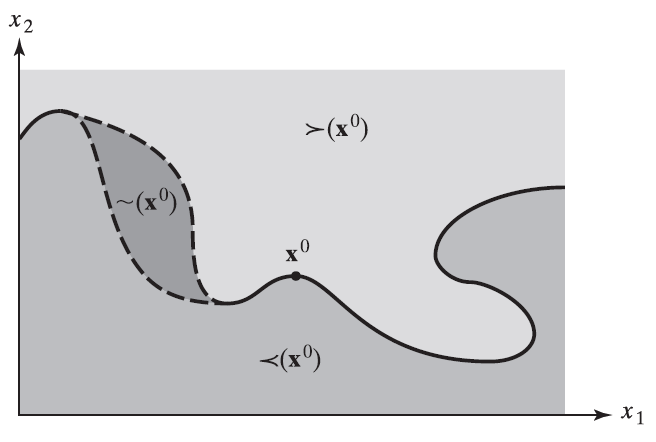
\includegraphics[width=0.8\textwidth]{1.open}
\captionof{figure}{Hypothetical preferences satisfying Axioms 1 and 2.}
\label{open}}

What happens around the "boundary"?

\begin{itemize}
\item Axiom 3. Continuity (define boundary)

$\succsim (x)$ and $\precsim (x)$ sets are closed in $R^n_+$ for $x \in R^n_+ $.
\end{itemize}

Once the boundary is properly defined, there is no sudden preference reversal any more.
Now the preference set looks like Figure \ref{fig:ball}

\vspace{2mm}

{\centering
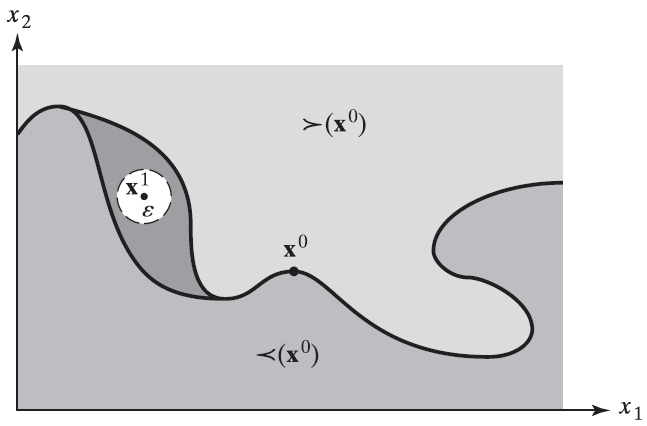
\includegraphics[width=0.8\textwidth]{1.ball}
\captionof{figure}{Hypothetical preferences satisfying Axioms 1, 2, and 3.}
\label{fig:ball}}

\vspace{2mm}

Further more, we assume "unlimited wants" can be represented by our preference.
For example, we can try Axiom 4'.

\begin{itemize}
\item Axiom 4'. Local non-satiation (always something better around)

$\forall \ x^0 \in R^n_+ \ $ and $ \ \forall \ \epsilon > 0$, $\exists x 
\in B_{\epsilon}(x^0) \cap R^n_+ \ $ s.t. $\ x \succ x^0$
\end{itemize}


Axiom 4' rulled out the "indifference zone" in Figure \ref{fig:ball} and our preference set
is deduced into Figure \ref{fig:line}.

{\centering
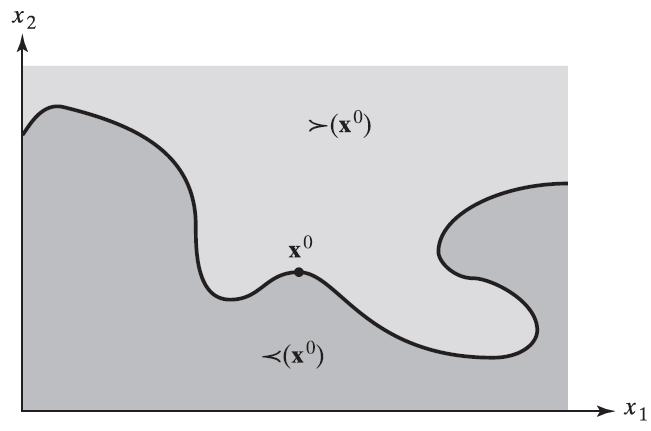
\includegraphics[width=0.8\textwidth]{1.line}
\captionof{figure}{Hypothetical preferences satisfying Axioms 1, 2, 3 and 4'}
\label{fig:line}}
\vspace{2mm}

However, Axiom 4' doesn't mean "the more, the better (at least not worse)" shown in Figure \ref{fig:mono}.

{\centering
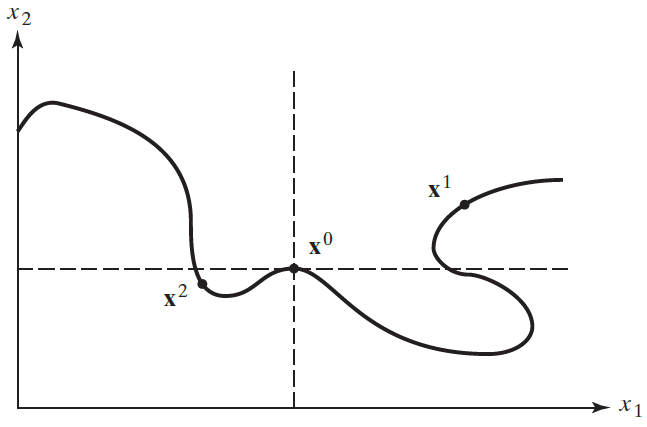
\includegraphics[width=0.8\textwidth]{1.mono}
\captionof{figure}{Hypothetical preferences satisfying Axioms 1, 2, 3 and 4' again}
\label{fig:mono}}
\vspace{2mm}

To depict this, we assume Axiom 4 instead.

\begin{itemize}
\item Axiom 4. Strict monotonicity (the more, the better)

$\forall \ x^0, x^1 \in R^n_+ \ $, if $x^0 \ge x^1, \ $ then  $\ x^0 \succsim x^1 \ $, while if 
$x^0 \gg x^1, \ $ then  $\ x^0 \succ x^1$.
\end{itemize}

A set of preferences satisfying Axioms 1, 2, 3, and 4 is given in Figure \ref{fig:closest}

{\centering
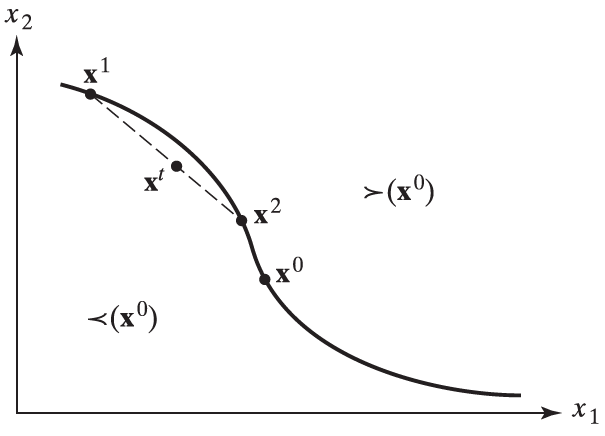
\includegraphics[width=0.8\textwidth]{1.closest}
\captionof{figure}{Hypothetical preferences satisfying Axioms 1, 2, 3 and 4}
\label{fig:closest}}
\vspace{2mm}

In addition, we assume people prefer "balanced" than "extreme" bundles in consumption.
Either Axiom 5' or Axiom 5 can guarantee this, but Axiom 5 will make our analysis easier in the future.


\begin{itemize}

\item Axiom 5'. Convexity

If $\ x^1 \succsim x^0 \ $, then $\ tx^1 + (1-t)x^0 \succsim x^0 \ $ for all $\ t \in [0,1]$

\item Axiom 5. Strict convexity

If $\ x^1 \ne x^0 \ $ and $\ x^1 \succsim x^0 \ $, then $\ tx^1 + (1-t)x^0 \succ x^0 \ $ for all $\ t \in (0,1)$

\end{itemize}





\end{mdframed}



%%%%%%%%%%%%%%%%%%%%%%%%%%%%%%%%%%%%%%%%%%%%%%%%%%%%%%%%%%%%%%%%%%%%%%%%%%%%%%%%%%%%%%%%%%%%%%

\section{Jehle \& Reny 1.9}

Sketch a map of indifference sets that are \textbf{all parallel right angles that ‘kink’ on the line $x_1 = x_2$}. If
\textbf{preference increases north-easterly}, these preferences will satisfy Axioms 1, 2, 3, and 4'. 

Prove that they also satisfy Axiom 5'. 

Do they satisfy Axiom 4? 

Do they satisfy Axiom 5?

%%%%%%%%%%%%%%%%%%%%%%%%%%%%%%%%%%%%%%%%%%%%%%%%%%%%%%%%%%%%%%%%%%%%%%%%%%%%%%%%%%%%%%%%%%%%%%
\section{Jehle \& Reny 1.13}
A consumer has lexicographic preferences over $x R2$ if the relation  satisfies $x_1, x_2$ whenever
$x_1^1 > x_1^2$, or $x_1^1 = x_1^2$ and $x_1^1 \ge x_1^2$.

(a) Sketch an indifference map for these preferences.

(b) Can these preferences be represented by a continuous utility function? Why or why not?

%%%%%%%%%%%%%%%%%%%%%%%%%%%%%%%%%%%%%%%%%%%%%%%%%%%%%%%%%%%%%%%%%%%%%%%%%%%%%%%%%%%%%%%%%%%%%%

\section{Jehle \& Reny 1.15}
Prove that the budget set, $B$, is a \textbf{compact, convex set whenever $p \gg 0$}.

%%%%%%%%%%%%%%%%%%%%%%%%%%%%%%%%%%%%%%%%%%%%%%%%%%%%%%%%%%%%%%%%%%%%%%%%%%%%%%%%%%%%%%%%%%%%%%

\section{Jehle \& Reny 1.26}
A consumer of \textbf{two goods} faces \textbf{positive prices} and has a \textbf{positive income}. 
His utility function is $$u(x_1, x_2) = x_1$$ 

Derive the Marshallian demand functions.

%%%%%%%%%%%%%%%%%%%%%%%%%%%%%%%%%%%%%%%%%%%%%%%%%%%%%%%%%%%%%%%%%%%%%%%%%%%%%%%%%%%%%%%%%%%%%%

\section{Jehle \& Reny 1.27}
A consumer of \textbf{two goods} faces \textbf{positive} prices and has a \textbf{positive income}. 
His utility function is $$u(x_1, x_2) = max[ax_1, ax_2] + min[x_1, x_2], \ \ where \ \ 0 < a < 1.$$
Derive the Marshallian demand functions.


\end{document}